% Основная часть работы. Введение и заключение желательно сюда не пихать, вынося в отдельные файлы
\chapter{Постановка задачи}

\textbf{Цель:}
Изучение и программирование робота на мобильной дифференциальной платформе.

\textbf{Исходные данные:}
\begin{enumerate}
	\item Вспомогательная литература по основам робототехники.
	\item Вспомогательная литература по основам схемотехники и электротехники.
	\item Вспомогательная литература по программированию микроконтроллеров на языке python.
	\item Мобильная платформа Eurobot Жук с набором различных датчиков.
\end{enumerate}

\textbf{Задачи:}
\begin{enumerate}
	\item Ознакомиться с учебной литературой и восполнить академическую разницу.
	\item Выбрать рабочую конфигурацию робота.
	\item Создать программу на ЯП python для движения по данным с энкодеров.
	\item Написать отчёт по проделанной работе.
\end{enumerate}

\chapter{Фукнциональные требования к роботу}

\begin{enumerate}
	\item Система должна иметь два режима управления: ручной, автоматический.
	\item В автоматическом режиме система должна иметь возможность передвигаться на основе данных, получаемых с датчиков.
	\item В ручном режиме робот должен иметь возможность принимать команды из REPL.
\end{enumerate}

\chapter{Конструкция}
\section{Шасси}

Шасси --- это ключевой элемент любого мобильного устройства, которая отвечает за его подвижность и общую функциональность. Оно представляет собой совокупность механических и структурных компонентов, которые обеспечивают передачу механической энергии от двигателей к активным элементам движения, таким как колеса или гусеницы.

Как было сказано выше, робот передвигается на дифференциальной платформе. Данный тип шасси был выбран в силу простоты программирования и конструкции, а также надёжности. При всех преимуществах такой конструкции она имеет довольно низкую проходимость, но для учебного робота это абсолютно некритично.

По совокупности характеристик были выбраны моторы GA25-370. Из-за низкой массы робота и ограниченного пространства колёса подключены к моторам напрямую. Сами моторы управляются через драйвер L9110S. Колёса состоят из лёгких пластиковых дисков, которые имеют такие плюс как дешевизна и простота изготовления, а также резиновых шин, обеспечивающих хорошее сцепление с поверхностью.

Таким образом обеспечивается подвижность изделия в достаточном объёме.

\section{Манипулятор}

Манипулятор --- это важный узел, позволяющий роботу взаимодействовать с окружающими объектами.

В случае Жука работа манипулятора обеспечивается двумя сервомоторами MG90D, которые являются удобным и надежным
решением для выполнения задач, не требующих больших нагрузок.

Клешни манипулятора являются сменными и на данный момент не установлены.

Таким образом робот имеет всё необходимое для лёгкой модификации и адаптации к новым задачам, требующим операций внешними объектами.

\section{Корпус}

Корпус --- это важная часть любого изделия, требуемая для защиты и

У робота есть несущий корпус, который обеспечивает лёгкость и компактность конструкции, а также достаточную защиту всех элементов. Он имеет небольшие габариты и вес, простоту управления и высокую точность поворота.

Выглядит корпус как полый цилиндр, внутри которого находятся все важные компоненты и создан с помощью аддитивных технологий. Сверху и снизу корпус закрыт пластинами, предположительно текстолитовыми или алюминьевыми. Для упрощения обслуживания и сборки внутри корпуса есть разделительная пластина. В нижней части находятся тяжёлые аккумуляторы и моторы для максимально низкого расположения центра масс и увеличения устойчивости робота. В верхней расположена лёгкая электроника, что позволяет с минимальными усилиями менять конфигурацию периферийных устройств, подключённых к микроконтроллеру.

Кроме этого верхняя половина корпуса содержит:
\begin{itemize}
	\item Отверстие для кнопки питания.
	\item Отверстие для разъема miceoUSB-B, необходимого при подзарядке и прошивке.
	\item Специальные места для винтов, обеспечивающие прочное соединение корпуса и крышек.
\end{itemize}

Нижняя половина корпуса тоже имеет технологические особенности. Предусмотрены:
\begin{itemize}
	\item Колодцы для колес, обеспечивающих мобильность системы.
	\item Отверстия для ультразвуковых датчиков.
	\item Места для крепления крышки и разделительной пластины.
\end{itemize}


Таким образом обеспечиваются защита от различных неблагоприятных факторов и упорядочивание важных деталей робота.

\section{Аддитивные технологии}

Аддитивные технологии, или аддитивное производство, --- это метод создания трехмерных объектов путем послойного добавления материала. В отличие от традиционных методов, таких как механическая обработка, где материал удаляется, аддитивное производство позволяет создавать сложные формы и конструкции с высокой детализацией.

В рамках проекта была использована технология 3D печати, которая зарекомендовала себя как один из наиболее эффективных методов для создания прототипов индивидуальных деталей и моделей.
Данный выбор обусловлен доступностью технологии, относительно низкой стоимостью, а так же возможностью создания уникальных элементов, которые были необходимы в проекте, причём с достаточно высокой точностью.

Использование аддитивных технологий в разработке этих незаменимых компонентов позволило достичь необходимого расположения деталей и обеспечить их функциональность. Благодаря высокой точности 3D печати удалось создать корпус, который полностью соответствует требованиям проекта и обеспечивает надежную работу всех систем.

\chapter{Электроника}

\section{ESP-WROOM-32}

ESP-WROOM-32 --- это микроконтроллер, который сочетает в себе Wi-Fi и Bluetooth. Основные характеристики приведены ниже:

\begin{description}
    \item[Частота процессора]: 80 МГц - 240 МГц
    \item[Память]: 4 МБ внешней SPI флеш-памяти
    \item[Bluetooth]: v4.2 BR/EDR и BLE
    \item[Операционное напряжение]: 3.0 В - 3.6 В
    \item[Средний ток потребления]: 80 мА
    \item[Минимальный ток питания]: 500 мА
    \item[Температурный диапазон]: -40 °C до +85 °C
    \item[Интерфейсы]: UART, SPI, I2C, SDIO, GPIO и другие
    \item[Встроенные датчики]: датчик Холла, температурный датчик
\end{description}

Эти характеристики вкупе с низкой стоимостью делают ESP-WROOM-32 идеальным выбором для разработки учебного робота.

\section{MPU 6050 (гироскоп)(GY-521)}
\begin{figure}[!h]
    \includegraphics[width=0.95\linewidth]{./graphics/img/mpu_6050.png}
    \caption{MPU 6050}
    \label{f:MPU_6050}
\end{figure}

MPU-6050 --- это модуль, который сочетает в себе 3-осевой гироскоп и 3-осевой акселерометр, позволяя определять положение и движение робота в пространстве. В списке ниже представлены его основные характеристики:

\begin{description}
    \item[Питание:] 3.5 - 6 В
    \item[Ток потребления:] 500 мкА
    \item[Интерфейс связи:] I2C
    \item[Размеры:] 2.0 см x 1.6 см x 0.3 см
    \item[Вес:] 5 г
\end{description}

Из приведённого выше ясно, что данный модуль подходит для проекта идеально.

\section{Электромоторы с энкодерами GA25-370}
\begin{figure}[!t]
	\includegraphics[width=0.95\linewidth]{graphics/img/GA25-370.jpg}
	\caption{Мотор-редуктор GA25-370}
	\label{f:GA25_370}
\end{figure}

GA25-370 --- это мощный DC-редукторный мотор, который широко используется в робототехнике и других приложениях, требующих высокого крутящего момента. Ниже приведены его основные характеристики:

\begin{description}
    \item[Рабочее напряжение:] 6V / 12V DC
    \item[Ток (без нагрузки):] 0.07A - 0.1A
    \item[Ток (нагрузка):] 0.3A - 0.5A
    \item[Ток (застревание):] 1.8A - 2.2A
    \item[Мощность:] 3W
    \item[Скорость (без нагрузки при 12V):] 350 об/мин
    \item[Скорость (нагрузка при 12V):] 245 об/мин
    \item[Вес:] около 100g
\end{description}

Таким образом данные моторы оказываются отличным выбором для лёгкой мобильной платформы.

\begin{figure}[!h]
    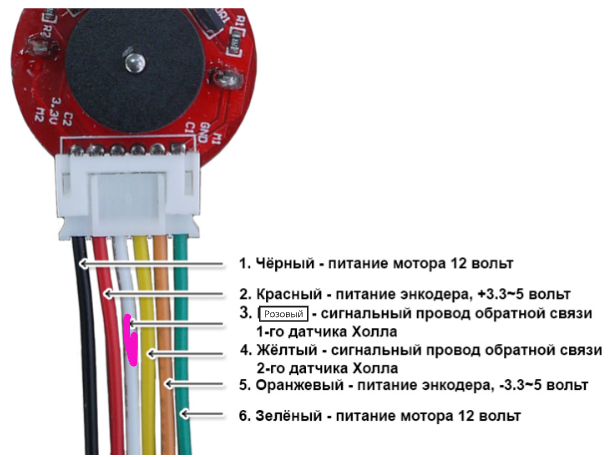
\includegraphics[width=0.7\linewidth]{./graphics/img/encoder_pinout.png}
    \caption{Распиновка энкодеров}
    \label{f:enc_pinout}
\end{figure}
\begin{figure}[!h]
    \includegraphics[width=0.7\linewidth]{./graphics/img/mini-L298N.jpg}
    \caption{Драйвер mini-L298N}
    \label{f:L298N}
\end{figure}

Двигатели подключены к остальной системе через энкодеры по шести проводам, значение которых показано на картинке \ref{f:enc_pinout}

Также важно сказать, что двигатели и энкодеры подключаются через аналоговые пины и управление происходит просто подачей напряжения на соответствующие выходы без дополнительных библиотек. Для снижения нагрузки на линии питания микроконтроллера используется драйвер L298N, показанный на рисунке \ref{f:L298N}.

Сам же GA25-370 изображен на рисунке \ref{f:GA25_370}

\section{УЗ-датчики HC SR04}
\begin{figure}[!h]
    \includegraphics[width=0.95\linewidth]{./graphics/img/HC-SR04.jpg}
    \caption{HC SR04}
    \label{f:HC_SR04}
\end{figure}

HC-SR04 --- это ультразвуковой датчик расстояния, который используется для определения расстояния до объекта с помощью звуковых волн. Как и ранее, важнейшие характеристики собраны в список.

\begin{description}
    \item[Рабочее напряжение:] 5V DC
    \item[Рабочий ток:] 15mA
    \item[Минимальное расстояние измерения:] 2cm
    \item[Максимальное расстояние измерения:] 400cm
    \item[Точность измерения:] ±3mm
    \item[Угол измерения:] <15°
    \item[Сигнал выхода эха:] TTL pulse, пропорциональный расстоянию
    \item[Размеры:] 45mm x 20mm x 15mm
\end{description}

Основываясь на этих данных, можно сказать, что этот датчик идеально подходит для различных проектов в области робототехники и автоматизации.

\begin{figure}[!h]
    \includegraphics[width=0.95\linewidth]{./graphics/img/HC-SR04_principe.png}
    \caption{Принцип работы УЗ датчика}
    \label{f:HC_SR04_prnc}
\end{figure}

Принцип работы HC-SR04 основан на использовании ультразвуковых волн. Передатчик датчика генерирует ультразвуковой импульс, который отражается от препятствия и регистрируется приемником. Микроконтроллер измеряет время, за которое импульс был отправлен и получен обратно, и на основе этого времени вычисляет расстояние до препятствия.На рисунке \ref{f:HC_SR04_prnc} представлена схема этого процесса.

\section{Micro servo MG90D}
\begin{figure}[!h]
    \includegraphics[width=0.95\linewidth]{./graphics/img/MG90D.png}
    \caption{MG90D}
    \label{f:MG90D}
\end{figure}

MG90D --- это цифровой сервопривод с металлическими шестернями, который часто используется в радиоуправляемых моделях и робототехнике. Ниже можно увидеть его основные характеристики:

\begin{description}
    \item[Рабочее напряжение:] 4.8V - 6.6V
    \item[Ток (без нагрузки):] 15mA
    \item[Ток (нагрузка):] до 500mA
    \item[Размеры:] 22.8 mm x 12.2 mm x 28.5 mm
    \item[Вес:] 13g
\end{description}

Таким образом данный сервопривод оптимален для манипулятора.

\chapter{Программная разработка}
\section{MicroPython}

MicroPython --- это интерпретируемый язык программирования, основанный на Python. Отличается наличием библиотек для управления микроконтроллерами и некоторыми оптимизациями для большей производительности. Был выбран по историческим причинам и из-за личных предпочтений.

Альтернативой является язык Arduino. Он основан на C++ и обладает многими его плюсами и минусами. Так этот ЯП является компилируемым, что делает несколько более сложной отладку кода и перепрошивку микроконтроллера, но гарантирует отличную производительность. Из-за того, что сложных вычислений на роботе Жук не предполагается, использовать данный язык программирования будет нерационально.

Для правильной работы необходимо прошить МК. В рамках этой работы были использованы встроенные средства Thonny. При этом есть альтернативные способы, описание которых можно найти в открытых источниках.

\subsection{Окружение}
Для работы с кодом использовалась IDE Thonny, установленная в виртуальное окружение для Python. Создаётся виртуальное окружение последовательностью команд в терминале:

{\tt
    \noindent\hangindent=5mm\hangafter=1
    mkdir /path/to/project/directory/ \# здесь создаётся директория (папка) в котой будут храниться файлы проекта. Команда зависит от ОС (приведён пример для linux) и имеет аналоги в граф. интерфейсе.

    \noindent\hangindent=5mm\hangafter=1
    cd /path/to/project/directory/ \# переход в рабочую директорию. Команда зависит от ОС (приведён пример для linux) и обязана исполняться в командой строке

    \noindent\hangindent=5mm\hangafter=1
    venv venv \# команда, которая создаёт в текущей директории папку venv и автоматически генерирует в ней необходимые файлы

}
\noindent Для активации venv надо запустить скрипт \texttt{activate}. Например:\\
\texttt{
    source /path/to/project/directory/venv/bin/activate
}\\
Сама IDE устанавливается командой \texttt{pip install thonny} внутри активированного venv.

Все библиотеки рекомендуется устанавливать локально в окружение текущего проекта, что я и сделал с помощью той же команды \texttt{pip install}.

\subsection{Библиотеки}
Как было сказано ранее, важной особенностью выбранного ЯП является сильное разбиение на библиотеки, поэтому работу следует начинать как раз с выбора этих пакетов.

На основании использованных компонентов были выбраны следующие библиотеки:
\begin{description}
    \item[machine] --- встроенная библиотека для работы с микроконтроллером и его периферийными устройствами.\\
    Документация: https://docs.micropython.org/en/latest/library/ machine.html
    \item[utime] --- встроенная библиотека для работы с таймерами и датой.\\
    Документация: https://docs.micropython.org/en/latest/library/ utime.html
    \item[machine.I2C] --- встроенный класс для работы с интерфейсом I2C.\\
    Документация: https://docs.micropython.org/en/latest/library/ machine.I2C.html
    \item[pcf8574] --- сторонняя библиотека для работы с расширителем пинов PCF8574.\\
    Документация: https://github.com/mcauser/micropython-pcf8574
    \item[mpu6050] --- сторонняя библиотека для работы с гироскопом MPU-6050.\\
    Документация: https://github.com/adamjezek98/ MPU6050-ESP8266-MicroPython
    \item[sr04] --- сторонняя библиотека для работы с УЗ-датчиками HRC SR04.\\
    Документация: https://github.com/rsc1975/micropython-hcsr04
\end{description}

Таким образом в дальнейшей работе надо обратить пристальное внимание на упомянутые библиотеки для работы с sr04, pcf8574, временем, а также machine для работы с самим МК.

\subsection{Движение}

Ниже приведён отрывок кода, который выключает моторы. У моторов в данной конструкции робота есть всего 3 состояния: вперёд, назад и выключены. Чтобы поменять направление движения, надо поменять у всех пинов IN на OUT и наоборот.

{\ttfamily
\begin{verbatim}
    from machine import Pin


    pin_l1 = Pin(2, Pin.IN)
    pin_l2 = Pin(15, Pin.OUT)
    pin_r1 = Pin(4, Pin.IN)
    pin_r2 = Pin(0, Pin.OUT)

    pin_l2.value(0)
    pin_r2.value(0)
\end{verbatim}
}
